\documentclass[11pt]{article}
\usepackage{amsmath,amssymb,amsthm,enumitem}
\usepackage{algorithm}
\usepackage[noend]{algpseudocode}
\usepackage[margin=1in]{geometry}
\usepackage[normalem]{ulem}
\usepackage{float}
\usepackage{graphicx}
\usepackage{setspace}
\usepackage{textcomp}
\usepackage{verbatim}
\usepackage{mathtools}
\usepackage{enumitem}
\usepackage{complexity}
\usepackage{tikz}
\usepackage{cleveref}
\restylefloat{table}
\usetikzlibrary{automata, positioning, arrows}
\useunder{\uline}{\ul}{}

\title{\bf  \\[2ex]
\rm\normalsize Charles Bolton}
\date{}
\author{}

\makeatletter
\def\BState{\State\hskip-\ALG@thistlm}
\makeatother

\begin{document}

\tikzset{->, >=stealth, every state/.style={thick, fill=gray!10, initial text=$ \textbf{start}$}, node distance=3cm}

\paragraph{Problem 1:} The proof that the $\sqrt{2} \notin \mathbb{Q}$ is the seed for proving irrationality of other integer roots, whose proofs techniques seem to take advantage of two main techniques; we'll look at both.\\\indent Both techniques tread the path taken by the $\sqrt{2}$ proof before diverging. For the first, assume two irreducible co-prime integers $a$ and $b$: 

\begin{align}
\sqrt[]{3} &= \frac a b \\
3 &= \frac{a^2}{b^2} \\
3b^2 &= a^2 \\
\therefore 3 \> | \> a^2 &\implies 3 \> | \> a \\
\therefore a &= 3c \\
 3b^2 &= (3c)^2 \\
3b^2 &= 9c^2 \\
b^2 &= 3c^2 \\
\therefore 3 \> | \> b^2 &\implies 3 \> | \> b \\
\perp &(1)
\end{align}
\setcounter{equation}{3} 

(1) sets up the problem (for contradiction), (2) squares both sides, (3) multiplies both by $b^2$. (4) says that 3 divides $a^2$ which comes from (3). This also means that 3 divides $a$ by recognizing that since $a$ is irreducible, $a^2$ is necessarily a multiplication of prime factors that come from $a$. This means we can replace a with a $3$ times some number $c$ (5) and substitute this value in (3) to get (6) and (7). Algebra gives us a contradiction with (1) at (10) because we found that both $a$ and $b$ are both reducible. To prove the bonus question for all primes $p$, recycle the same proof but replace $3$ and $3^2$ with $p$ and $p^2$ and the contradiction again arises. \\\indent The other technique goes to step (3) and then examines two cases. In the first, we assume $b$ is even, so $3b^2$ and $a^2$ are also even, which leads to the same contradiction in the $\sqrt 2$ proof. So case two chooses odd $b$, which means $3b^2$ and $a^2$ are odd. By some algebraic trickery, we can exchange each odd number with another number such that:
\begin{align}
b &= 2p + 1\\
a &= 2q + 1\\
3(2p +1)(2p+1) &= (2q + 1)(2q + 1) \qquad \text{from}\>(3, 4, 5)\\
3(4p^2 + 4p + 1) &= 4q^2 + 4q + 1\\
12p^2 + 12p + 3 &= 4q^2 + 4q + 1\\
12p^2 + 12p + 2 &= 4q^2 + 4q\\
2(6p^2 + 6p + 1) &= 2(2q^2 + 2q)\\
6p^2 + 6p + 1 &= 2q^2 + 2q\\
&\perp
\end{align}   

Here the contradiction comes from (3, 4, 5, 11) where we can see that both sides have contradictory parity, with the left side odd and the right side even. 

\paragraph{Problem 2:} For the inductive proof, we start with a base case $|A| = 1$ then $|P(A)| =  2^1 = 2$. The elements of the power set of the singleton set are the empty set and the single element. We choose to start with $n = 1$ as per the prompt (assume $n \geq 1$ throughout) so we have the proof sketch: \\

(1) The set $A_1 = \{x\}$ and $\mathcal{P}(A_1) = \{x, \{\}\}$\\
\indent(2) Show $|A_1| = 1$ and $|\mathcal{P}(A_1)| = 2^1 = 2$ \qquad\qquad\qquad\\
\indent (3) Assume $|A_n| = n \implies |\mathcal{P}(A_n)| = 2^n$\\
\indent (4) Show $|A_{n+1}| = n + 1 \implies |\mathcal{P}(A_{n+1})| = 2^{n+1} $\\
\indent (5) $|\mathcal{P}(A_{n+1})| = 2^n \cdot 2 $ \\
\indent (6) $|\mathcal{P}(A_{n+1})| = |\mathcal{P}(A_n)| \cdot 2 $ \\
\indent (7) $A_{n+1} = A_n \cup \{y \>| \>y \notin A_n\}$\\
\indent (8) $|\mathcal{P}(A_{n+1})| = |\mathcal{P}(A_n \cup\{y\})|$ \\

We need to show (5), that the cardinality of the power set is multiplied by two each time a new element is added to the set. Since the power set of $A_n$ is the set of all sets in $A_n$, when we add a new element $y$ to $A_n$ we need to also add the union of that element with every subset already in the power set of $A_n$ to get the power set $A_{n+1}$. Since the union of an element with the empty set (from $A_n$) is just the element itself, we can count one union for every subset already in $A_n$, doubling the amount of subsets. A way to visualize this is to think of all the $2^n$ subsets in $A_n$ as nodes in a graph with zero edges. Suppose you added a new node that was connected by a single edge to every other node in the graph. You would have $2^n$ edges, representing the newly added subsets.

\paragraph{Problem 3:} The average human head has approximately 100,000 hair follicles. Assume a higher maximum follicle number such that the amount of hairs on a single human head is bounded by the range [0, 200,000]. Meanwhile, the population of the United States is approximately 327 million people, each of whom possesses (for the sake of argument) one head. Suppose we found 200,000 people who miraculously each had one more hair than the previous, such that if we lined them up we would have one person at the beginning with 0 hairs, the second person with 1 hair, the third with 2 (and so on) and the person at the end with exactly 200,000 hairs, our upper bound (no person can have more hairs on their head). Next, suppose we added one more person to our sample size, such that we had 200,001 specimen. By the pigeon-hole principle (ie, there are more people in our total population size than hair follicles), the 200,001$^{st}$ person would have to have a hair-count in the allowed range, meaning s/he would have the exact same amount of hairs as another person in the sample. Therefore, it is true that there exist two people in the United States with the same amount of hairs on their respective heads.\\
\indent The proof can be extended to 100 people by the following reasoning. We can assign each person to one of 200,000 holes, corresponding to the amount of hairs on their head. Notice that once we have exceeded 200,000 people, we have necessarily found at least one match. In fact, each time we have a multiple of 200,000 people added to the holes, we would have at least one more match. If each person were assigned to the next hole (modulo 200,000), there would be around 1600 people in each hole (divide 327 million by 200 thousand), meaning that not only are there definitely 100 people with the same amount of hairs on their heads, but there are at least 1600 people with the exact same amount of hairs. The actual number of people with the exact same amount of hairs is likely much higher, since such an even distribution at the extremes is unlikely, and we would probably see a more normal distribution about the mean. 

\paragraph{Problem 4:} The way to prove that the cardinality of the set of binary strings of countably infinite length is uncountably infinite is to use Cantor's diagonalization method. First, we need to arrange a table of all the infinitely long binary strings in a table, such that each next binary string is arranged directly below the previous string. These strings can be arranged in any order, as long as each next string is different than all the strings that came before it. As an example table, we could have the following: \\

\begin{table}[h]
\begin{tabular}{ll|l|l|l|l|l|l|l|l|l|l|l|l|l|}
\cline{3-15}
1  &  & {\ul \textbf{1}} & 1                & 1                & 1                & 1                & 1                & 1                & 1                & 1                & 1                & 1                & 1                & ... \\ \cline{3-15} 
2  &  & 0                & {\ul \textbf{0}} & 0                & 0                & 0                & 0                & 0                & 0                & 0                & 0                & 0                & 0                & ... \\ \cline{3-15} 
3  &  & 1                & 0                & {\ul \textbf{1}} & 0                & 1                & 0                & 1                & 0                & 1                & 0                & 1                & 0                & ... \\ \cline{3-15} 
4  &  & 0                & 1                & 0                & {\ul \textbf{1}} & 0                & 1                & 0                & 1                & 0                & 1                & 0                & 1                & ... \\ \cline{3-15} 
4  &  & 1                & 1                & 0                & 0                & {\ul \textbf{1}} & 1                & 0                & 0                & 1                & 1                & 0                & 0                & ... \\ \cline{3-15} 
6  &  & 0                & 0                & 1                & 1                & 0                & {\ul \textbf{0}} & 1                & 1                & 0                & 0                & 1                & 1                & ... \\ \cline{3-15} 
7  &  & 1                & 1                & 1                & 0                & 0                & 0                & {\ul \textbf{1}} & 1                & 1                & 0                & 0                & 0                & ... \\ \cline{3-15} 
8  &  & 0                & 0                & 0                & 1                & 1                & 1                & 0                & {\ul \textbf{0}} & 0                & 1                & 1                & 1                & ... \\ \cline{3-15} 
9  &  & 1                & 0                & 0                & 1                & 0                & 0                & 1                & 0                & {\ul \textbf{0}} & 1                & 0                & 0                & ... \\ \cline{3-15} 
10 &  & 0                & 1                & 1                & 0                & 1                & 1                & 0                & 0                & 1                & {\ul \textbf{1}} & 0                & 0                & ... \\ \cline{3-15} 
11 &  & 1                & 0                & 1                & 1                & 1                & 0                & 1                & 0                & 1                & 1                & {\ul \textbf{1}} & 0                & ... \\ \cline{3-15} 
12 &  & 0                & 1                & 0                & 0                & 0                & 1                & 0                & 1                & 0                & 0                & 0                & {\ul \textbf{1}} & ... \\ \cline{3-15} 
\end{tabular}
\end{table}
Each string in the table is infinitely long (denoted by the ellipses) and the vertical height is also infinitely tall. Notice the numbers on the left, providing a one-to-one correspondence between the natural positive integers and the set of binary strings. This correspondence shows that the set of binary strings is countably infinite. Of course, the dagger is on the diagonal. Cantor's method tells us that we can create another binary string by taking the bit in each of the diagonal positions from top left to bottom right (in bold and underlined) and flip the bit, thus guaranteeing that this string differs from every other string in the infinite set of strings. So in the example, our bit string would be 010001011000... The objection one often makes when initially looking at this proof is to claim that the diagonal string would eventually show up in an infinite set of binary strings, and indeed, we could append our set with this newly discovered string. But then we could just flip the bit on the diagonal again and we'd have a new string. This shows that there exist elements outside of the infinite set itself, and that no matter how we arrange our set to include every string, strings of infinite length will still not be described by, or be members of, the set of infinitely long binary strings. Therefore, the cardinality of this set is uncountable. 

\paragraph{Problem 5:} 
We will show that the triple prime conjecture is false by observing several repeating patterns and properties that are always true of candidate members of this set which exclude them from the set. Indeed, not only is this set not infinite, but there is only 1 element of this set of triple-primes. It helps to arrange all the candidate triple primes in a vertical table like the one on the following page. From the table, we can observe a few patterns. First, there are 5 different `types' of candidate elements. After we add 2 to any of these numbers five times, we've added 10 and we repeat the same pattern, incrementing the tens digit. So each set of 5 three-tuples is ten more than the previous.

\begin{table}[H]
\begin{tabular}{lllllll}
\hline
1  & 3  & 5  &    &    &    &    \\ \hline
   & 3  & 5  & 7  &    &    &    \\ \hline
   &    & 5  & 7  & 9  &    &    \\ \hline
   &    &    & 7  & 9  & 11 &    \\ \hline
   &    &    &    & 9  & 11 & 13 \\ \hline
11 & 13 & 1\textbf{5} &    &    &    &    \\ \hline
   & 13 & 1\textbf{5} & 17 &    &    &    \\ \hline
   &    & 1\textbf{5} & 17 & 19 &    &    \\ \hline
   &    &    & 17 & 19 & 21 &    \\ \hline
   &    &    &    & 19 & 21 & 23 \\ \hline
21 & 23 & 2\textbf{5} &    &    &    &    \\ \hline
   & 23 & 2\textbf{5} & 27 &    &    &    \\ \hline
   &    & 2\textbf{5} & 27 & 29 &    &    \\ \hline
   &    &    & 27 & 29 & 31 &    \\ \hline
   &    &    &    & 29 & 31 & 33 \\ \hline
31 & 33 & 3\textbf{5} &    &    &    &    \\ \hline
   & 33 & 3\textbf{5} & 37 &    &    &    \\ \hline
   &    & 3\textbf{5} & 37 & 39 &    &    \\ \hline
   &    &    & 37 & 39 & 41 &    \\ \hline
   &    &    &    & 39 & 41 & 43 \\ \hline
41 & 43 & 4\textbf{5} &    &    &    &    \\ \hline
   & 43 & 4\textbf{5} & 47 &    &    &    \\ \hline
   &    & 4\textbf{5} & 47 & 49 &    &    \\ \hline
   &    &    & 47 & 49 & 51 &    \\ \hline
   &    &    &    & 49 & 51 & 53 \\ \hline
51 & 53 & 5\textbf{5} &    &    &    &    \\ \hline
   & 53 & 5\textbf{5} & 57 &    &    &    \\ \hline
   &    & 5\textbf{5} & 57 & 59 &    &    \\ \hline
   &    &    & 57 & 59 & 61 &    \\ \hline
   &    &    &    & 59 & 61 & 63 \\ \hline
61 & 63 & 6\textbf{5} &    &    &    &    \\ \hline
   & 63 & 6\textbf{5} & 67 &    &    &    \\ \hline
   &    & 6\textbf{5} & 67 & 69 &    &    \\ \hline
   &    &    & 67 & 69 & 71 &    \\ \hline
   &    &    &    & 69 & 71 & 63 \\ \hline
71 & 73 & 7\textbf{5} &    &    &    &    \\ \hline
   & 73 & 7\textbf{5} & 77 &    &    &    \\ \hline
   &    & 7\textbf{5} & 77 & 79 &    &    \\ \hline
   &    &    & 77 & 79 & 81 &    \\ \hline
   &    &    &    & 79 & 81 & 83 \\ \hline
81 & 83 & 8\textbf{5} &    &    &    &    \\ \hline
   & 83 & 8\textbf{5} & 87 &    &    &    \\ \hline
   &    & 8\textbf{5} & 87 & 89 &    &    \\ \hline
   &    &    & 87 & 89 & 91 &    \\ \hline
   &    &    &    & 89 & 91 & 93 \\ \hline
91 & 93 & 9\textbf{5} &    &    &    &    \\ \hline
   & 93 & 9\textbf{5} & 97 &    &    &    \\ \hline
   &    & 9\textbf{5} & 97 & 99 &    &    \\ \hline
\end{tabular}
\end{table}

For the following elimination discussion, we are not including the first two triple-primes $\{ 1, 3, 5 \}, \{3 ,5, 7\}$ (the first is not a triple-prime because it contains 1 and the second is the only triple-prime) or the third  $\{5, 7, 9\}$ (which fails because it has a 9 in it). \\

Begin by eliminating multiples of 5. After the first 5 three-tuples, each successive set of 5 three-tuples begins with three three-tuples which include one element whose last digit is 5. We can eliminate all 3 of these tuples for the entire (infinite) table because each contains an element divisible by 5 and hence is of course not prime. Since we are adding 10 each time we wrap to a new set, we will never fail to find a number which has a 5 as a last digit in the first three tuples. Eliminating, we get:
\begin{table}[H]
\begin{tabular}{llll}
\hline
7  & \textbf{9}  & 11 &    \\ \hline
   & \textbf{9}  & 11 & 13 \\ \hline
17 & 19 & 21 &    \\ \hline
   & 19 & 21 & 23 \\ \hline
27 & 29 & 31 &    \\ \hline
   & 29 & 31 & 33 \\ \hline
37 & 39 & 41 &    \\ \hline
   & 39 & 41 & 43 \\ \hline
47 & 49 & 51 &    \\ \hline
   & 49 & 51 & 53 \\ \hline
57 & 59 & 61 &    \\ \hline
   & 59 & 61 & 63 \\ \hline
67 & 69 & 71 &    \\ \hline
   & 69 & 71 & 63 \\ \hline
77 & 79 & 81 &    \\ \hline
   & 79 & 81 & 83 \\ \hline
87 & 89 & 91 &    \\ \hline
   & 89 & 91 & 93 \\ \hline
\end{tabular}
\end{table}

The next observation we can make is that, of the remaining two types, the first contains numbers whose \textit{last digits} are [7, 9, 1] respectively and the second type contains numbers with [9, 1, 3] as the last digit of each. Since we add 10 each time we wrap the set, this will be the case to infinity.\\

For the next step, we can show that every three-tuple contains exactly one composite number in the following way. Notice that 9 is composite in the first line. Eliminate the first line and the one below it, because the 9s stack. For the proof, we create the resulting table with line numbers below.


\begin{table}[H]
\begin{tabular}{lllll}
\cline{2-5}
1  & 17 & 19 & 21 &    \\ \cline{2-5} 
2  &    & 19 & 21 & 23 \\ \cline{2-5} 
3  & 27 & 29 & 31 &    \\ \cline{2-5} 
4  &    & 29 & 31 & 33 \\ \cline{2-5} 
5  & 37 & 3\textbf{9} & 41 &    \\ \cline{2-5} 
6  &    & 3\textbf{9} & 41 & 43 \\ \cline{2-5} 
7  & 47 & 49 & 51 &    \\ \cline{2-5} 
8  &    & 49 & 51 & 53 \\ \cline{2-5} 
9  & 57 & 59 & 61 &    \\ \cline{2-5} 
10 &    & 59 & 61 & 63 \\ \cline{2-5} 
11 & 67 & 6\textbf{9} & 71 &    \\ \cline{2-5} 
12 &    & 6\textbf{9} & 71 & 63 \\ \cline{2-5} 
13 & 77 & 79 & 81 &    \\ \cline{2-5} 
14 &    & 79 & 81 & 83 \\ \cline{2-5} 
15 & 87 & 89 & 91 &    \\ \cline{2-5} 
16 &    & 89 & 91 & 93 \\ \cline{2-5} 
\end{tabular}
\end{table}

Next, we can see that every line numbered $6n$ or $6n-1 \> \forall n \geq 1$ can be eliminated because it contains number whose last digit is divisible by 3. This can be shown mathematically. First, observe that line 6 and 5 (6-1) each contain 39. Since 39 can be broken up as 39 = 30 + 9, we know it is divisible by 3, since both 30 and 9 are divisible by 3. Every 6$^{th}$ set of 2 three-tuples contains a number $30n +9$ because we add 30 each time, maintaining divisibility by 3.

\begin{table}[H]
\begin{tabular}{lllll}
\cline{2-5}
1  & 17 & 19 & 2\textbf{1} &    \\ \cline{2-5} 
2  &    & 19 & 2\textbf{1} & 23 \\ \cline{2-5} 
3  & 27 & 29 & 31 &    \\ \cline{2-5} 
4  &    & 29 & 31 & 33 \\ \cline{2-5} 
7  & 47 & 49 & 5\textbf{1} &    \\ \cline{2-5} 
8  &    & 49 & 5\textbf{1} & 53 \\ \cline{2-5} 
9  & 57 & 59 & 61 &    \\ \cline{2-5} 
10 &    & 59 & 61 & 63 \\ \cline{2-5} 
13 & 77 & 79 & 8\textbf{1} &    \\ \cline{2-5} 
14 &    & 79 & 8\textbf{1} & 83 \\ \cline{2-5} 
15 & 87 & 89 & 91 &    \\ \cline{2-5} 
16 &    & 89 & 91 & 93 \\ \cline{2-5} 
\end{tabular}
\end{table}

We can continue in this fashion, by noting that every line numbered ($6n - 5$) and $(6n - 4)$ contains a number which ends in a 1 and is divisible by 3, since $21 + 30n$ is likewise always divisible by 3. This leaves us with the last two types below.

\begin{table}[H]
\begin{tabular}{lllll}
\cline{2-5}
3  & 2\textbf{7} & 29 & 31 &    \\ \cline{2-5} 
4  &    & 29 & 31 & 3\textbf{3} \\ \cline{2-5} 
9  & 5\textbf{7} & 59 & 61 &    \\ \cline{2-5} 
10 &    & 59 & 61 & 6\textbf{3} \\ \cline{2-5} 
15 & 8\textbf{7} & 89 & 91 &    \\ \cline{2-5} 
16 &    & 89 & 91 & 9\textbf{3} \\ \cline{2-5} 
\end{tabular}
\end{table}

Continue another time with lines numbered $(6n - 3)$ because each contains a number that is $27 +30n$. Lines numbered $(6n - 2)$ all contain a number $33 + 30n$. Algebraically, we have now eliminated every single candidate element because we have eliminated every candidate element whose line number corresponds to a multiple 6 or every number between each multiple of 6.

\paragraph{Problem 6:} 
We can use Cantor's diagonal method to show that the interval (0, 1) is uncountably infinite. In addition, there exist certain functions that map every member of $\mathbb{R}$ to the interval (0,1). To map the real numbers to the interval, we can choose the continuous, infinite on-the-interval and asymptotic-at-the-bounds piecewise function $f(x) =$ 


\[ \begin{cases} 
      -tan(\frac{\pi}{2}-\frac{\pi  x}{2})+2 & x < 1/2 \\
      tan(\frac{\pi  x}{2}) & x\geq 1/2 \\
   \end{cases}
\]

Next we need to find a mapping from the real numbers to the interval; we can choose the function $g(x)$ which is the inverse of the first function divided by two: 

\begin{align*}
	   \frac{(tan^{-1}(x-2)+\frac{\pi}{2})}{\pi} 
\end{align*} 
  
With these two function we can show that a bijection exists between the reals and the interval. 

\paragraph{Problem 7:} 

From the lone axiom $MI$ we can only get two strings (theorems) using rules 1 and 2:
\setcounter{equation}{0} 

\begin{align}
MI&[1]--> MIU\\ 
MI&[2]--> MII 
\end{align}  
Using rule 1 and then repeating rule 2 on $MII$ we can derive $M(IIU)^n$. Using rule 2 on $MIU$, we can derive $M(IU)^n$:

\begin{align}
MII &[1]n--> M+(IIU)*2^n\\ 
MIU &[2]n--> M+(IU)*2^n
\end{align}  

We can ignore all strings of the form on the right side (3)(4) because they are not useful in reducing the string to $MU$. That is, it isn't possible to get anything else out of these strings using the rules. This is because for both, the string ends in $IIU$ or $IU$ and once we have a single $U$ ending a string, the rules don't allow us to derive anything but duplicating the part after $M$ because there are no $III$ or $UU$ substrings. \\
\indent Next, we can focus on strings derived from (2) $MII$. Repeatedly applying rule 2:

\begin{align}
MII &[2]n--> M+(II)*2^n
\end{align} 
From this we can continually apply rule 3  and rule 4 (if we have $UU$) to the end of the string to get back to (1), which doesn't help us. This is because, for every $III$ that we remove from the end of (5), we get

\begin{align}
M+2^n(II)-3(III)
\end{align} 
Mathematically, we will always end up with the axiom $MIU$ or the string $MII$ doing this because $2^n-3k \>\> \forall k \geq 1$ will always either be odd or even matching the parity of $k$. If $n$ is odd, we can reduce to $MI$ and if $n$ is even, we can reduce to $MII$. We can prove this inductively: 
 
\begin{align*}
2^1 &= 2 \\
\therefore \quad (3k \>&\nmid 2^1)\\
Assume \qquad (3k \>&\nmid 2^{n})\\
\therefore \> case \>1: \quad &2^n = 3k+1 \\ ||case \> 2: \quad &2^n = 3k+3 \\
\therefore \qquad &2^{n+1} = 2(3k+1) = 6k+2 \\
 || \quad &2^{n+1} = 2(3k+2) = 6k+4 = 6k+3+1 \\
\end{align*}
This lemma simply shows that $3k$ can never divide $2^n$ and therefore the equation $2^n-3k = 0$ is unsolvable. Therefore we will never end up with the string $MU$, we will always end up with either $MIU$ or $MII$. But we're not done. \\
\indent We can also have the string $MUI$ by applying [3] to the front of $MIIII$ from (5). Here again we are stuck either appending $IU$ or doubling $UI$.\\
\indent Finally, we can also have an infinite amount of strings of the form $M+I^{+}+\{U^*, I^*\}$ by applying [3] to (6) in various ways to reach strings which have any number of $U$ between some number of $I$. But notice that we always have an $I$ at the beginning of these strings, and that we have already shown we can't mathematically to get from $MI$ to (5) to $MU$ so the same lemma applies in this situation as well. Namely, we can always reduce down to $MIU$ or $MII$, but because we can't get the right multiples of 3 and 2, we'll never get $MU$. 

\paragraph{Questions from the Sipser Text:} 

\paragraph{1.3} \mbox{}\\\\

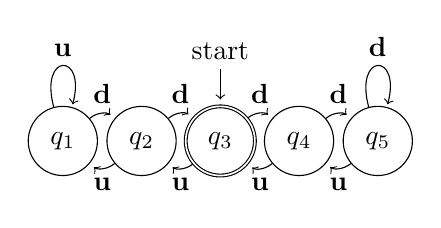
\begin{tikzpicture}
	[shorten >=2pt, on grid,auto] 
   \node[state] (q_1)   {$q_1$}; 
   \node[state] (q_2) [right=of q_1] {$q_2$}; 
   \node[state,initial above=40,accepting](q_3) [right=of q_2] {$q_3$};
   \node[state] (q_4) [right=of q_3] {$q_4$};
   \node[state] (q_5) [right=of q_4] {$q_5$};
    \path[->] 
    (q_1) edge [loop above=40] node {$\textbf{u}$} (q_1)
          edge [bend left=40] node {$\textbf{d}$} (q_2)
    (q_2) edge [bend left=40] node {$\textbf{u}$} (q_1)
          edge [bend left=40] node {$\textbf{d}$} (q_3)
    (q_3) edge [bend left=40] node {$\textbf{u}$} (q_2)
          edge [bend left=40] node {$\textbf{d}$} (q_4)
    (q_4) edge [bend left=40] node {$\textbf{u}$} (q_3)
          edge [bend left=40] node {$\textbf{d}$} (q_5)
    (q_5) edge [bend left=40] node {$\textbf{u}$} (q_4)
          edge [loop above] node {$\textbf{d}$} (q_5);
\end{tikzpicture}

\paragraph{1.6} \mbox{}\\\\
\textbf{a.} Begin with 1, end with a 0\\
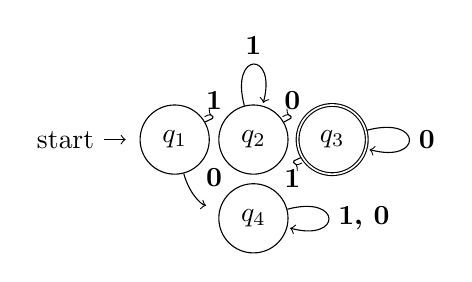
\begin{tikzpicture}
	[shorten >=5pt, on grid,auto] 
   \node[state, initial] (q_1)   {$q_1$}; 
   \node[state] (q_2) [right=of q_1] {$q_2$}; 
   \node[state, accepting](q_3) [right=of q_2] {$q_3$};
   \node[state] (q_4) [below right=of q_1] {$q_4$};
    \path[->] 
    (q_1) edge [bend right=30] node {$\textbf{0}$} (q_4)
          edge [bend left=30] node {$\textbf{1}$} (q_2)
    (q_2) edge [loop above=30] node {$\textbf{1}$} (q_1)
          edge [bend left=30] node {$\textbf{0}$} (q_3)
    (q_3) edge [bend left=30] node {$\textbf{1}$} (q_2)
          edge [loop right=30] node {$\textbf{0}$} (q_4)
    (q_4) edge [loop right=30] node {$\textbf{1, 0}$} (q_3);
\end{tikzpicture}
\mbox{}\\\\\\    
\noindent \textbf{d.} Length at least 3, third symbol a 0\\
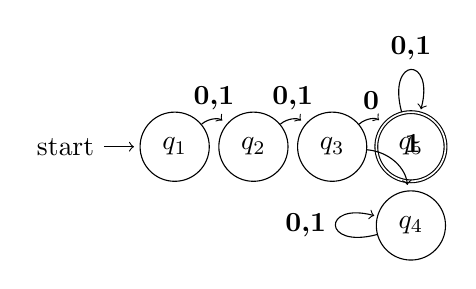
\begin{tikzpicture}
	[shorten >=2pt, on grid,auto] 
   \node[state, initial] (q_1)   {$q_1$}; 
   \node[state] (q_2) [right=of q_1] {$q_2$}; 
   \node[state](q_3) [right=of q_2] {$q_3$};
   \node[state] (q_4) [below right=of q_3] {$q_4$};
   \node[state, accepting] (q_5) [right=of q_3] {$q_5$};
    \path[->] 
    (q_1) edge [bend left=40] node {$\textbf{0,1}$} (q_2)
    (q_2) edge [bend left=40] node {$\textbf{0,1}$} (q_3)
    (q_3) edge [bend left=40] node {$\textbf{1}$} (q_4)
    		  edge [bend left=40] node {$\textbf{0}$} (q_5)	
    (q_4) edge [loop left=40] node {$\textbf{0,1}$} (q_4)
    (q_5) edge [loop above] node {$\textbf{0,1}$} (q_5);
\end{tikzpicture}

\mbox{}\\\\  
\noindent \textbf{g.} Length at most 5\\\\
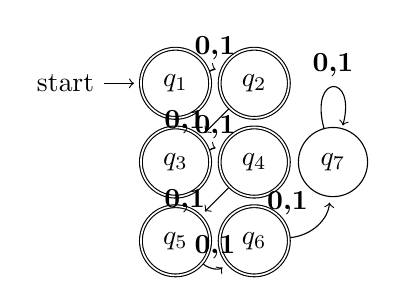
\begin{tikzpicture}
	[shorten >=2pt, on grid,auto] 
   \node[state, initial, accepting] (q_1)   {$q_1$}; 
   \node[state, accepting] (q_2) [right=of q_1] {$q_2$}; 
   \node[state, accepting](q_3) [below left=of q_2] {$q_3$};
   \node[state, accepting] (q_4) [right=of q_3] {$q_4$};
   \node[state, accepting] (q_5) [below left=of q_4] {$q_5$};   
   \node[state, accepting] (q_6) [right=of q_5] {$q_6$};
   \node[state] (q_7) [above right=of q_6] {$q_7$};

    \path[->] 
    (q_1) edge [bend left=20] node {$\textbf{0,1}$} (q_2)
    (q_2) edge [left=40] node {$\textbf{0,1}$} (q_3)
    (q_3) edge [bend left=20] node {$\textbf{0,1}$} (q_4)
    (q_4) edge [left=40] node {$\textbf{0,1}$} (q_5)        
    (q_5) edge [bend right=40] node {$\textbf{0,1}$} (q_6)
    (q_6) edge [bend right=40] node {$\textbf{0,1}$} (q_7)
    (q_7) edge [loop above] node {$\textbf{0,1}$} (q_7);
\end{tikzpicture}

\mbox{}\\\\  
\noindent \textbf{j.} At least two 0s, at most one 1 \\\\
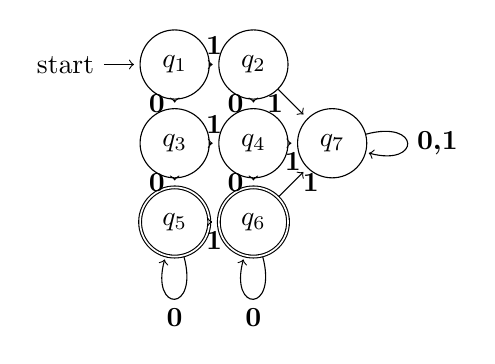
\begin{tikzpicture}
	[shorten >=2pt, on grid,auto] 
   \node[state, initial] (q_1)   {$q_1$}; 
   \node[state] (q_2) [right=of q_1] {$q_2$}; 
   \node[state] (q_3) [below=of q_1] {$q_3$};
   \node[state] (q_4) [right=of q_3] {$q_4$};
   \node[state, accepting] (q_5) [below=of q_3] {$q_5$};   
   \node[state, accepting] (q_6) [right=of q_5] {$q_6$};
   \node[state] (q_7) [right=of q_4] {$q_7$};

    \path[->] 
    (q_1) edge [above=20] node {$\textbf{1}$} (q_2) 
    (q_1) edge [left=20] node {$\textbf{0}$} (q_3)
    (q_2) edge [left=40] node {$\textbf{0}$} (q_4)
    (q_2) edge [left=40] node {$\textbf{1}$} (q_7)
    (q_3) edge [above=20] node {$\textbf{1}$} (q_4)
    (q_3) edge [left=20] node {$\textbf{0}$} (q_5)
    (q_4) edge [left=40] node {$\textbf{0}$} (q_6)     
    (q_4) edge [below=40] node {$\textbf{1}$} (q_7)     
    (q_5) edge [below=40] node {$\textbf{1}$} (q_6)
    (q_5) edge [loop below] node {$\textbf{0}$} (q_5)
    (q_6) edge [loop below] node {$\textbf{0}$} (q_6)
    (q_6) edge [right =40] node {$\textbf{1}$} (q_7)
    (q_7) edge [loop right] node {$\textbf{0,1}$} (q_7);
\end{tikzpicture}

\mbox{}\\\\  
\noindent \textbf{n.} All strings except empty \\\\
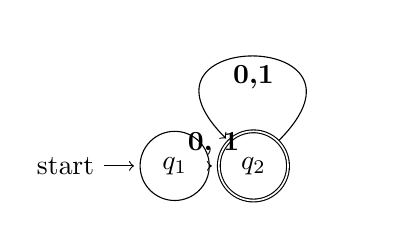
\begin{tikzpicture}
	[shorten >=2pt, on grid,auto] 
   \node[state, initial] (q_1)   {$q_1$}; 
   \node[state, accepting] (q_2) [right=of q_1] {$q_2$}; 

    \path[->] 
    (q_1) edge [above=20] node {$\textbf{0, 1}$} (q_2) 
    (q_2) edge [loop] node {$\textbf{0,1}$} (q_1);

\end{tikzpicture}

\mbox{}\\\\  
\noindent \textbf{1.11} In order to turn a given NFA into an NFA with only one accept state, simply create a new accept state $q_{accept}$ and add $\epsilon$ edges to $q_{accept}$ from all existing accept states and revoke their accepting nature. Now, $q_{accept}$ is the only accepting state in the NFA, but the NFA is the same as the one it was derived from, since adding epsilon edges in this way will not change the strings that either NFA  accepts.\\\\

\paragraph{1.16} \mbox{}\\\\
\textbf{a.} After removing unreachable states, we have the following DFA:\\\\
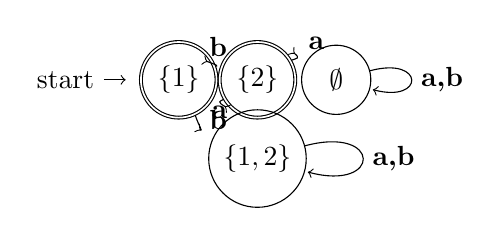
\begin{tikzpicture}
	[shorten >=5pt, on grid,auto] 
   \node[state, initial, accepting] (q_1)   {$\{1\}$}; 
   \node[state, accepting] (q_2) [right=of q_1] {$\{2\}$}; 
   \node[state](q_3) [right=of q_2] {$\emptyset$};
   \node[state] (q_4) [below right=of q_1] {$\{1,2\}$};
    \path[->] 
    (q_1) edge [bend right=20] node {$\textbf{a}$} (q_4)
          edge [bend left=20] node {$\textbf{b}$} (q_2)
    (q_2) edge [bend left=30] node {$\textbf{b}$} (q_1)
          edge [bend left=30] node {$\textbf{a}$} (q_3)
    (q_3) 
          edge [loop right=30] node {$\textbf{a,b}$} (q_4)
    (q_4) edge [loop right=30] node {$\textbf{a,b}$} (q_3);
\end{tikzpicture}
\mbox{}\\\\
\textbf{b.} After removing unreachable states, we have the following DFA:\\\\
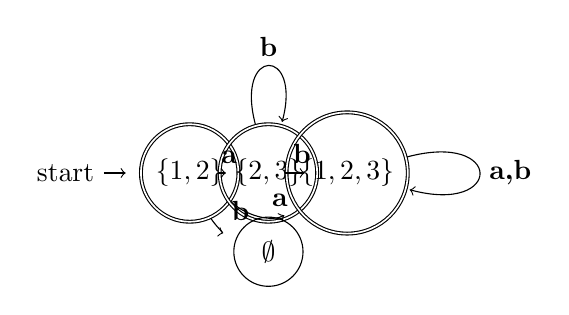
\begin{tikzpicture}
	[shorten >=5pt, on grid,auto] 
   \node[state, initial, accepting] (q_1)   {$\{1, 2\}$}; 
   \node[state, accepting] (q_2) [right=of q_1] {$\{2,3\}$}; 
   \node[state, accepting](q_3) [right=of q_2] {$\{1, 2, 3\}$};
   \node[state] (q_4) [below right=of q_1] {$\emptyset$};
    \path[->] 
    (q_1) edge [bend right=20] node {$\textbf{b}$} (q_4)
          edge [bend right=35] node {$\textbf{a}$} (q_3)
    (q_2) edge [loop above=30] node {$\textbf{b}$} (q_1)
          edge [above=30] node {$\textbf{a}$} (q_1)
    (q_3) edge [above=30] node {$\textbf{b}$} (q_2)
          edge [loop right=30] node {$\textbf{a,b}$} (q_3);
\end{tikzpicture}

\paragraph{1.19} \mbox{}\\

\noindent \textbf{a.}$(0 \cup 1)^*000(0\cup1)^*$\\

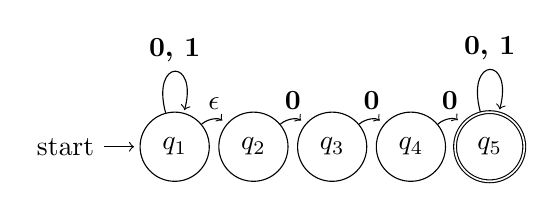
\begin{tikzpicture}
	[shorten >=2pt, on grid,auto] 
   \node[state, initial] (q_1)   {$q_1$}; 
   \node[state] (q_2) [right=of q_1] {$q_2$}; 
   \node[state] (q_3) [right=of q_2] {$q_3$};
   \node[state] (q_4) [right=of q_3] {$q_4$};
   \node[state, accepting] (q_5) [right=of q_4] {$q_5$};
    \path[->] 
    (q_1) edge [loop above] node {$\textbf{0, 1}$} (q_1)
          edge [bend left=40] node {$\epsilon$} (q_2)
    (q_2) 
          edge [bend left=40] node {$\textbf{0}$} (q_3)
    (q_3) 
          edge [bend left=40] node {$\textbf{0}$} (q_4)
    (q_4) 
          edge [bend left=40] node {$\textbf{0}$} (q_5)
    (q_5) edge [loop above] node {$\textbf{0, 1}$} (q_5);
\end{tikzpicture}

\mbox{}\\\\
\textbf{b.} $(((00)^*(11))\cup 01)^*$\\

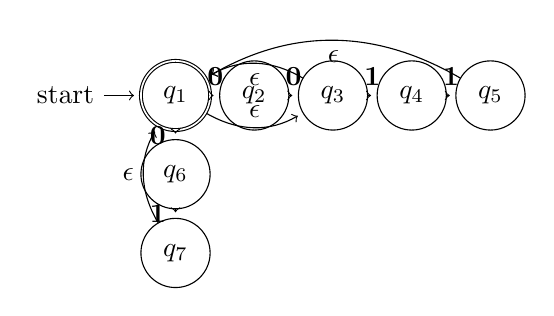
\begin{tikzpicture}
	[shorten >=2pt, on grid,auto] 
   \node[state, initial, accepting] (q_1)   {$q_1$}; 
   \node[state] (q_2) [right=of q_1] {$q_2$}; 
   \node[state] (q_3) [right=of q_2] {$q_3$};
   \node[state] (q_4) [right=of q_3] {$q_4$};
   \node[state] (q_5) [right=of q_4] {$q_5$};
   \node[state] (q_6) [below=of q_1] {$q_6$};
   \node[state] (q_7) [below=of q_6] {$q_7$};
    \path[->] 
    (q_1) 
          edge [above=40] node {$\textbf{0}$} (q_2)
          edge [bend right=30] node {$\epsilon$} (q_3)
          edge [left=40] node {$\textbf{0}$} (q_6)
    (q_2) 
          edge [above=40] node {$\textbf{0}$} (q_3)
          
    (q_3) 
          edge [above=40] node {$\textbf{1}$} (q_4)
          edge [bend right=30] node {$\epsilon$} (q_1)
    (q_4) 
          edge [above=40] node {$\textbf{1}$} (q_5)
    (q_5) edge [bend right=30] node {$\epsilon$} (q_1)
    (q_6) edge [left=40] node {$\textbf{1}$} (q_7)
    (q_7) edge [bend left=30] node {$\epsilon$} (q_1);
\end{tikzpicture}

\mbox{}\\\\
\textbf{c.}  $\emptyset^*$

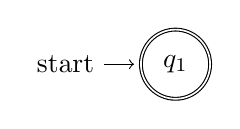
\begin{tikzpicture}
	[shorten >=2pt, on grid,auto] 
   \node[state, initial, accepting] (q_1)   {$q_1$}; 
    \path[->] ;
\end{tikzpicture}

\paragraph{1.20} Strings following `are' are accepted and strings following `not' are not accepted.
\mbox{}\\
\textbf{a.} are: $ab$, $aab$ not: $ba$, $baa$\\
\textbf{b.} are: $ab$, $abab$ not: $b$, $ba$\\
\textbf{c.} are: $a$, $b$ not: $ab$, $aba$\\
\textbf{d.} are: $aaa$, $aaaaaa$ not: $b$, $bb$\\
\textbf{e.} are: $aba$, $aabaa$ not: $bbb$, $bab$\\
\textbf{f.} are: $aba$, $bab$ not: $a$, $b$\\
\textbf{g.} are: $b$, $ab$ not: $ba$, $bb$\\
\textbf{h.} are: $a$, $bb$ not: $b$, $\epsilon$\\\\ 

\paragraph{1.29} 
\mbox{}\\\textbf{a.} $A_1 = \{0^n1^n2^n \mid n\geq 0\}$\\ 

Choose $s = 0^p1^p2^p$. Using the PL, we can see a few possible cases for the string $xyz$. Since $|xy|\leq p$, we can see that $xy$ must be a string of zeros. Then, $xyyz$ would have more 0s than 1s or 2s. If $xy$ consisted of all 1s, we could have more 1s than 0s or 2s. The same argument applies if $y$ consists of all 2s. \\\indent The only other option has $y$ getting the order of the 0s, 1s, and 2s, jumbled up. This would happen if $y$ consisted of more than one alphabet symbol, because in this case $y^2$ would have a 0 following a 1 or a 2 or both, a 1 following a 2, etc.  

\mbox{}\\\textbf{b.} $A_2 = \{www \mid w\in \{a, b\}^*\}$\\\

Choose $s = ab^pab^pab^p$. The PL tells us that $s$ must be able to be broken up into $xyz$. Since $|xy| \leq p$, we know that $xy$ consists of $ab^n | n \leq p-1$ and $z$ consists of $b^{p-n}ab^pab^p$. The PL also states that each $xy^iz \in A_2$. Next we can break $xy$ up into $x = ab^m$, $y= b^{n-m}$. Then, for the string $xyyz$, we would have $ab^mb^{2(n-m)}b^{p-n}ab^pab^p = ab^{(2n-m-n+p)}ab^pab^p = ab^{(n-m)+p}ab^pab^p$. We know that $|y| = b^{n-m} > 0$. This means that for sufficiently large $i$,  $y^i$ has more than $p$ $b$s which means the string is not in the language. Another possibility, though, is if $|x| = 0$. In this case, we would have $y=ab^n$ and we would still wind up with string $ab^{n+p}ab^pab^p$ with more than $p$  $b$s in the first $w$.

\mbox{}\\\textbf{c.} $A_3 = \{a^{2^n} |n \geq 0\}$.\\\\ Choose $s= a^{2^p}$. Then, $xyz$ would consist of a string $a^n$ in $xy$ where $|xy|, n\leq p$ as well as a string of $a^{2^p-n}$ in $z$. Since $|xy| \leq p < 2^p$, $|xy| < 2^p$ and $|xyy| \leq y+y < 2^p + 2^p$. But $|xyyz| > 2^p$ since the PL states that $|y| > 0$. This allows strings whose length lies in between powers of 2, since $2^p >|xyyz| < 2^p + 2^p$. Answer admittedly ripped right out the book I can't figure out another way.\\\

\paragraph{1.30} \mbox{}\\

The simplest DFA for the language consists of a start state which has a self loop on 0 and a transition to a single accept state on 1 with a self loop on 1. The reason the proof doesn't work is because  the language doesn't require we have the same amount of 0s and 1s. So if we choose $s = 0^p1^p$, we have $xyz$ such that $|xy| \leq p$, $|y| > 0$. Going through the same cases for the proof in 1.73, we can have $y$ consists of \textbf{1}. only 0s, \textbf{2}. only 1s, or \textbf{3}. a combination of 1s and 0s. For \textbf{1}, $xyyz$ will have more 0s than 1s. Not a problem! For \textbf{2}, we will have more 1s than 0s. Again, not a problem. Finally for \textbf{3}, we just apply rules 2 and 3 of the PL, which say that  $|xy| \leq p$, $|y| > 0$, so we actually can't have $y$ be a mix of 0s and 1s, since $|0^p| = p$ so we would violate the rules to include a 1. Therefore, the PL applies to $s$ and the language is regular. Hence, the proof is incorrect.\\ 
\paragraph{1.36} \mbox{}\\\\
The problem suggests a language $B_n$ which contains all strings whose length is a multiple of $n$ concatenations of the string $a$. We know that if a language is indeed regular, it can also be described by an equivalent DFA. For the following, we have $\{n*k \mid n,k \in \mathbb{Z}^+\}$ (This means we can't have a string of length zero). To show that $B_n$ is regular, we first construct the following DFAs for $n = 1, 2, 3$ respectively: \\\\

\noindent 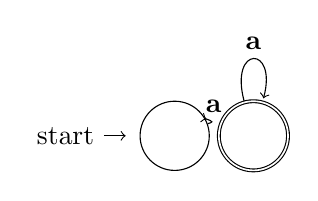
\begin{tikzpicture}
	[shorten >=5pt, on grid,auto] 
   \node[state, initial] (q_1)   {}; 
   \node[state, accepting] (q_2)[right=of q_1]   {}; 
    \path[->] 
    (q_1)
          edge [bend left=20] node {$\textbf{a}$} (q_2)
    (q_2) 
          edge [loop above=30] node {$\textbf{a}$} (q_1);

\end{tikzpicture}
 
\noindent 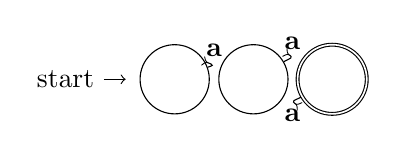
\begin{tikzpicture}
	[shorten >=5pt, on grid,auto] 
   \node[state, initial] (q_1)   {}; 
   \node[state] (q_2)[right=of q_1]   {}; 
   \node[state, accepting](q_3) [right=of q_2] {};
    \path[->] 
    (q_1)
          edge [bend left=20] node {$\textbf{a}$} (q_2)
    (q_2) 
          edge [bend left=30] node {$\textbf{a}$} (q_3)
    (q_3) edge [bend left=30] node {$\textbf{a}$} (q_2);

\end{tikzpicture}

\noindent 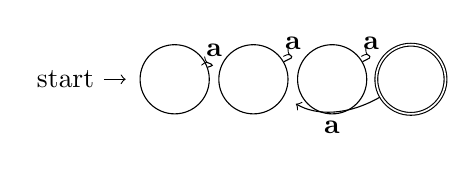
\begin{tikzpicture}
	[shorten >=5pt, on grid,auto] 
   \node[state, initial] (q_1)   {}; 
   \node[state] (q_2)[right=of q_1]   {}; 
   \node[state] (q_3)[right=of q_2]   {}; 
   \node[state, accepting](q_4) [right=of q_3] {};
    \path[->] 
    (q_1)
          edge [bend left=20] node {$\textbf{a}$} (q_2)
    (q_2) 
          edge [bend left=30] node {$\textbf{a}$} (q_3)
    (q_3) edge [bend left=30] node {$\textbf{a}$} (q_4)
    (q_4) edge [bend left=30] node {$\textbf{a}$} (q_2);
\end{tikzpicture}

We can go on in this way forever, constructing ever-longer DFAs that accept ever-larger $k$-multiples for each next $n$. From this observation, we can construct a GNFA from the union of all the above DFAs which will allow us to include all the DFAs which are equivalent to $B_n$ for some $n$. For example, from the first three DFAs above, we can union them, first adding a new start state, then a new accept state from all the original accept states: \\\\

\noindent 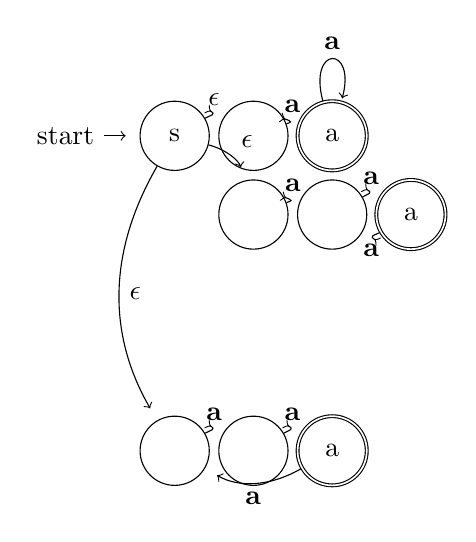
\begin{tikzpicture}
	[shorten >=5pt, on grid,auto] 
   \node[state, initial] (q_1)   {s}; 
   \node[state] (q_2)[below =4of q_1]   {}; 
   \node[state] (q_3)[right=of q_2]   {}; 
   \node[state, accepting](q_4) [right=of q_3] {a};
   \node[state] (q_5)[right=of q_1]   {};    
   \node[state, accepting] (q_6)[right=of q_5]   {a}; 
   \node[state] (q_7)[below right=of q_1]   {};     
   \node[state] (q_8)[right=of q_7]   {};    
   \node[state, accepting] (q_9)[right=of q_8]   {a}; 
    \path[->] 
    (q_1)
          edge [bend right=] node {$\epsilon$} (q_2)
          edge [bend left=] node {$\epsilon$} (q_5)
          edge [bend left=] node {$\epsilon$} (q_7)
    (q_2) 
          edge [bend left=30] node {$\textbf{a}$} (q_3)
    (q_3) edge [bend left=30] node {$\textbf{a}$} (q_4)
    (q_4) edge [bend left=30] node {$\textbf{a}$} (q_2)
    (q_5)
          edge [bend left=20] node {$\textbf{a}$} (q_6)
    (q_6) 
          edge [loop above=30] node {$\textbf{a}$} (q_6)
    (q_7)
          edge [bend left=20] node {$\textbf{a}$} (q_8)
    (q_8) 
          edge [bend left=30] node {$\textbf{a}$} (q_9)
    (q_9) edge [bend left=30] node {$\textbf{a}$} (q_8);
\end{tikzpicture}

\noindent \begin{tikzpicture}
	[shorten >=5pt, on grid,auto] 
   \node[state, initial] (q_1)   {s}; 
   \node[state] (q_2)[below=of q_7]   {}; 
   \node[state] (q_3)[right=of q_2]   {}; 
   \node[state](q_4) [right=of q_3] {};
   \node[state] (q_5)[right=of q_1]   {};    
   \node[state] (q_6)[right=of q_5]   {}; 
   \node[state] (q_7)[below right=of q_1]   {};     
   \node[state] (q_8)[right=of q_7]   {};    
   \node[state] (q_9)[right=of q_8]   {}; 
   \node[state, accepting] (q_10)[right=of q_9]   {a}; 
    \path[->] 
    (q_1)
          edge [bend right=20] node {$\epsilon$} (q_2)
          edge [bend left=20] node {$\epsilon$} (q_5)
          edge [bend left=20] node {$\epsilon$} (q_7)
    (q_2) 
          edge [bend left=20] node {$\textbf{a}$} (q_3)
    (q_3) edge [bend left=20] node {$\textbf{a}$} (q_4)
    		  		
    (q_4) edge [bend left=20] node {$\textbf{a}$} (q_2)
    	      edge [bend left=30] node {$\epsilon$} (q_10)
    (q_5)
          edge [bend left=20] node {$\textbf{a}$} (q_6)
    (q_6) 
          edge [loop above=20] node {$\textbf{a}$} (q_6)
          edge [bend left=20] node {$\epsilon$} (q_10)
    (q_7)
          edge [bend left=20] node {$\textbf{a}$} (q_8)
    (q_8) 
          edge [bend left=20] node {$\textbf{a}$} (q_9)
    (q_9) edge [bend left=20] node {$\textbf{a}$} (q_8)
    		  edge [bend left=20] node {$\epsilon$} (q_10);	
\end{tikzpicture}

Now we begin the process of ripping out states and recombining:\\

\noindent \begin{tikzpicture}
	[shorten >=5pt, on grid,auto] 
   \node[state, initial] (q_1)   {s}; 
   \node[state] (q_2)[below=of q_7]   {}; 
   \node[state] (q_3)[right=of q_2]   {}; 
   \node[state] (q_4) [right=of q_3] {};   
   \node[state] (q_6)[right=of q_5]   {}; 
   \node[state] (q_7)[below right=of q_1]   {};     
   \node[state] (q_8)[right=of q_7]   {};    
   \node[state] (q_9)[right=of q_8]   {}; 
   \node[state, accepting] (q_10)[right=of q_9]   {a}; 
    \path[->] 
    (q_1)
          edge [bend right=20] node {$\epsilon$} (q_2)
          edge [bend left=20] node {$\epsilon$} (q_6)
          edge [bend left=20] node {$\epsilon$} (q_7)
    (q_2) 
          edge [bend left=20] node {$\textbf{a}$} (q_3)
    (q_3) edge [bend left=20] node {$\textbf{a}$} (q_4)
    		  		
    (q_4) edge [bend left=20] node {$\textbf{a}$} (q_2)
    	      edge [bend left=30] node {$\epsilon$} (q_10)
    (q_6) 
          edge [loop above=20] node {$\textbf{a}^*$} (q_6)
          edge [bend left=20] node {$\epsilon$} (q_10)
    (q_7)
          edge [bend left=20] node {$\textbf{a}$} (q_8)
    (q_8) 
          edge [bend left=20] node {$\textbf{a}$} (q_9)
    (q_9) edge [bend left=20] node {$\textbf{a}$} (q_8)
    		  edge [bend left=20] node {$\epsilon$} (q_10);	

\end{tikzpicture}	

\noindent \begin{tikzpicture}
	[shorten >=5pt, on grid,auto] 
   \node[state, initial] (q_1)   {s}; 
   \node[state] (q_2)[below=of q_7]   {}; 
   \node[state] (q_3)[right=of q_2]   {}; 
   \node[state] (q_4) [right=of q_3] {};   
   \node[state] (q_6)[right=of q_5]   {};      
   \node[state] (q_9)[below=of q_6]   {}; 
   \node[state, accepting] (q_10)[right=of q_9]   {a}; 
    \path[->] 
    (q_1)
          edge [bend right=20] node {$\epsilon$} (q_2)
          edge [bend left=20] node {$\epsilon$} (q_6)
          edge [bend left=20] node {$\epsilon$} (q_9)
    (q_2) 
          edge [bend left=20] node {$\textbf{a}$} (q_3)
    (q_3) edge [bend left=20] node {$\textbf{a}$} (q_4)
    		  		
    (q_4) edge [bend left=20] node {$\textbf{a}$} (q_2)
    	      edge [bend left=30] node {$\epsilon$} (q_10)
    (q_6) 
          edge [loop above=20] node {$\textbf{a}^*$} (q_6)
          edge [bend left=20] node {$\epsilon$} (q_10)
    (q_9) edge [loop above=20] node {$\textbf{aa}^*$} (q_9)
    		  edge [bend left=20] node {$\epsilon$} (q_10);	

\end{tikzpicture}	
  
  \noindent \begin{tikzpicture}
	[shorten >=5pt, on grid,auto] 
   \node[state, initial] (q_1)   {s}; 
   \node[state] (q_2)[below=of q_7]   {};  
   \node[state] (q_6)[right=of q_5]   {};      
   \node[state] (q_9)[below=of q_6]   {}; 
   \node[state, accepting] (q_10)[right=of q_9]   {a}; 
    \path[->] 
    (q_1)
          edge [bend right=20] node {$\epsilon$} (q_2)
          edge [bend left=20] node {$\epsilon$} (q_6)
          edge [bend left=20] node {$\epsilon$} (q_9)
    (q_2) 
          edge [loop left=20] node {$\textbf{aaa}^*$} (q_2)
    	      edge [bend right=30] node {$\epsilon$} (q_10)
    (q_6) 
          edge [loop above=20] node {$\textbf{a}^*$} (q_6)
          edge [bend left=20] node {$\epsilon$} (q_10)
    (q_9) edge [loop above=20] node {$\textbf{aa}^*$} (q_9)
    		  edge [bend left=20] node {$\epsilon$} (q_10);	

\end{tikzpicture}
\mbox{}\\\\
    \noindent 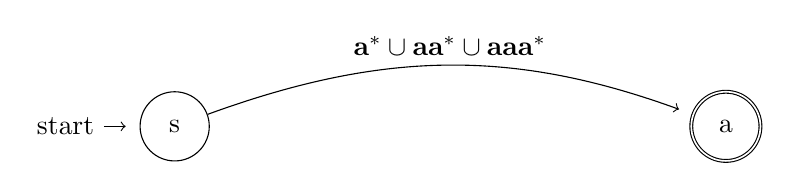
\begin{tikzpicture}
	[shorten >=5pt, on grid,auto, node distance = 7cm] 
   \node[state, initial] (q_1)   {s}; 
   \node[state, accepting] (q_10)[right=of q_1]   {a}; 
    \path[->] 
    (q_1)
    		  edge [bend left=20] node {$\textbf{a}^*\cup\textbf{aa}^* \cup\textbf{aaa}^*$} (q_10);	
\end{tikzpicture}

\mbox{}\\\\
From this we can generalize (further) the GNFA which accepts $B_n$ by doing this forever, so the arrow from start to accept would be $\textbf{a}^*\cup\textbf{aa}^* \cup\textbf{aaa}^* \cup ... \cup \textbf{a}^k$. Therefore, $B_n$ is regular. 

\paragraph{1.38} \mbox{}\\\\
One way to do this is to convert the \textbf{all}-NFA into a DFA, and then, instead of just making all states containing a state which is an accept state an accept state, also do the following: for every accept state, make each member of that accept state's set of states an accept state. So, if we refer to figure 1.44 in the Sipser text, you'd still have the same diagram, but the set of accept states would also include (for this example) the states with $\{2\}$, $\{3\}$ and the state with $\{2, 3\}$. Since we know that a language is regular if we can construct some FSM which will accept it, our work is done.

\paragraph{1.43} \mbox{}\\\\ 
The $DROP\-OUT$ operation is similar to (but not the same as) the reverse of a concatenation operation. Theorem 1.47 states that the class of regular languages is closed under the concatenation operation. To see why it is also closed under $DROP\-OUT$, first consider the following picture. For $\{x, z \in  \Sigma^* \}$, suppose we have 3 NFAs. The first, $N_1$, ends in an accept state after reading any string $x$ and the third, $N_3$, after reading any string $z$. The second NFA $N_2$ has a single start state with an arrow to another state on reading input $y$ (note that below $x$ and $z$ are strings that lead to accept states, whereas $y$ is just a character).

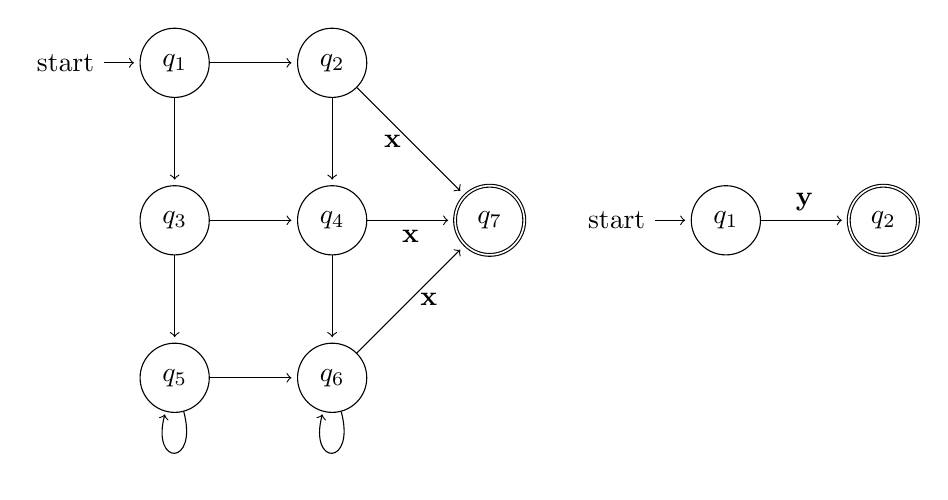
\begin{tikzpicture}
	[shorten >=2pt, on grid,auto, node distance=2cm] 
   \node[state, initial] (q_1)   {$q_1$}; 
   \node[state] (q_2) [right=of q_1] {$q_2$}; 
   \node[state] (q_3) [below=of q_1] {$q_3$};
   \node[state] (q_4) [right=of q_3] {$q_4$};
   \node[state] (q_5) [below=of q_3] {$q_5$};   
   \node[state] (q_6) [right=of q_5] {$q_6$};
   \node[state, accepting] (q_7) [right=of q_4] {$q_7$};
   \node[state, initial] (q_8) [right=3 of q_7] {$q_1$};
   \node[state, accepting] (q_9) [right=of q_8] {$q_2$};

    \path[->] 
    (q_1) edge [above=20] node {} (q_2) 
    (q_1) edge [left=20] node {} (q_3)
    (q_2) edge [left=40] node {} (q_4)
    (q_2) edge [left=40] node {$\textbf{x}$} (q_7)
    (q_3) edge [above=20] node {} (q_4)
    (q_3) edge [left=20] node {} (q_5)
    (q_4) edge [left=40] node {} (q_6)     
    (q_4) edge [below=40] node {$\textbf{x}$} (q_7)     
    (q_5) edge [below=40] node {} (q_6)
    (q_5) edge [loop below] node {} (q_5)
    (q_6) edge [loop below] node {} (q_6)
    (q_6) edge [right =40] node {$\textbf{x}$} (q_7)
    (q_8) edge [above =40] node {$\textbf{y}$} (q_9);
\end{tikzpicture}

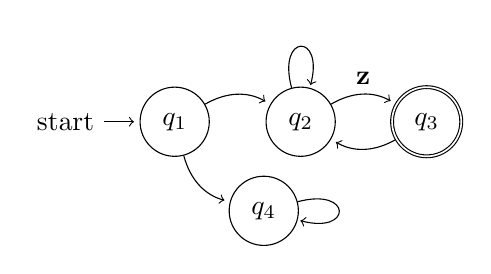
\begin{tikzpicture}
	[shorten >=2pt, on grid,auto, node distance=1.6cm] 
   \node[state, initial] (q_1)   {$q_1$}; 
   \node[state] (q_2) [right=of q_1] {$q_2$}; 
   \node[state, accepting](q_3) [right=of q_2] {$q_3$};
   \node[state] (q_4) [below right=of q_1] {$q_4$};
    \path[->] 
    (q_1) edge [bend right=30] node {} (q_4)
          edge [bend left=30] node {} (q_2)
    (q_2) edge [loop above=30] node {} (q_1)
          edge [bend left=30] node {$\textbf{z}$} (q_3)
    (q_3) edge [bend left=30] node {} (q_2)
    (q_4) edge [loop right=30] node {} (q_3);
\end{tikzpicture}
\mbox{}\\\\
We can concatenate these three NFAs using the construction in figure 1.48:\\\\

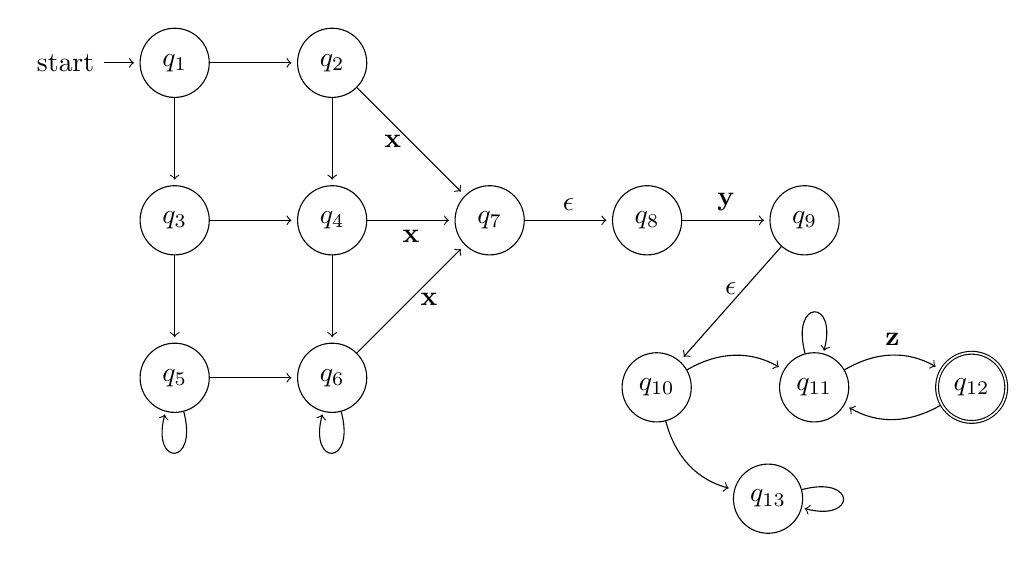
\begin{tikzpicture}
	[shorten >=2pt, on grid,auto, node distance=2cm] 
   \node[state, initial] (q_1)   {$q_1$}; 
   \node[state] (q_2) [right=of q_1] {$q_2$}; 
   \node[state] (q_3) [below=of q_1] {$q_3$};
   \node[state] (q_4) [right=of q_3] {$q_4$};
   \node[state] (q_5) [below=of q_3] {$q_5$};   
   \node[state] (q_6) [right=of q_5] {$q_6$};
   \node[state] (q_7) [right=of q_4] {$q_7$};
   \node[state] (q_8) [right=2 of q_7] {$q_8$};
   \node[state] (q_9) [right=of q_8] {$q_9$};
   \node[state] (q_10) [below right=3 of q_7]  {$q_{10}$}; 
   \node[state] (q_11) [right=of q_10] {$q_{11}$}; 
   \node[state, accepting](q_12) [right=of q_11] {$q_{12}$};
   \node[state] (q_13) [below right=of q_10] {$q_{13}$};

   \path[->] 
    (q_1) edge [above=20] node {} (q_2) 
    (q_1) edge [left=20] node {} (q_3)
    (q_2) edge [left=40] node {} (q_4)
    (q_2) edge [left=40] node {$\textbf{x}$} (q_7)
    (q_3) edge [above=20] node {} (q_4)
    (q_3) edge [left=20] node {} (q_5)
    (q_4) edge [left=40] node {} (q_6)     
    (q_4) edge [below=40] node {$\textbf{x}$} (q_7)     
    (q_5) edge [below=40] node {} (q_6)
    (q_5) edge [loop below] node {} (q_5)
    (q_6) edge [loop below] node {} (q_6)
    (q_7) edge [above] node {$\epsilon$} (q_8)
    (q_6) edge [right =40] node {$\textbf{x}$} (q_7)
    (q_8) edge [above =40] node {$\textbf{y}$} (q_9) 
    (q_9) edge [above =40] node {$\epsilon$} (q_10) 
    (q_10) edge [bend right=30] node {} (q_13)
          edge [bend left=30] node {} (q_11)
    (q_11) edge [loop above=30] node {} (q_10)
          edge [bend left=30] node {$\textbf{z}$} (q_12)
    (q_12) edge [bend left=30] node {} (q_11)
    (q_13) edge [loop right=30] node {} (q_13);

\end{tikzpicture}
 
From here it is easy to see that we can use the dropout operation on $N_2$ by ripping its states out and drawing an epsilon arrow from $q_7$ to $q_{10}$. Formally, \\

\noindent Let $N_1 = (Q_1, \Sigma, \delta_1, q_1, F_1)$ recognize $x$\\
\indent $N_2 = (Q_2, \Sigma, \delta_2, q_2, F_2)$ recognize $y$\\
\indent $N_3 = (Q_3, \Sigma, \delta_3, q_3, F_3)$ recognize $z$\\\\
Construct $N = (Q, \Sigma, \delta, q, F)$ to recognize $N_1 \circ N_2 \circ N_3$\\\\
\indent \textbf{1.} $Q = Q_1 \cup Q_2 \cup Q_3$\\
\indent \textbf{2.} The start state is the start state of $N_1$\\
\indent \textbf{3.} The accept state is the accept state of $N_3$\\
\indent \textbf{4.} Define $\delta$ such that all transitions are the same except those from accept states of $N_1$ and \indent\indent $N_2$, which now have epsilon transitions to start states of $N_2$ and $N_3$, respectively.\\
\indent \textbf{5.} $F$ is the set of accept states for $N_3$\\
\indent \textbf{6.} Remove the states of $N_2$.\\
\indent \textbf{7.} Add transitions from the accept states of $N_1$ to the start state of $N_3$\\

The NFA containing $y$ could contain many states, and the proof would still work. Therefore, regular languages are closed under $DROPOUT$.

\paragraph{1.45} \mbox{}\\\\ 	
If $A$ is regular, then there exists some DFA which describes the strings that $A$ accepts. If $wx \in A$ and $x \in B$, then there exists some string(s) $x \in A \cup B$ which, once concatenated onto $w \in A$ lead to some accept state in $A$. We can construct a new language $A \setminus B$ by finding the states in $A$ which we end up in after reading input $w$. For these states, some of them will lead to an accept state on $x$. Make these the new accept states and make the states that were accept states from these states on $x$ into non-accepting states.  

\paragraph{1.60} \mbox{}\\\\ 

The following NFA demonstrates one example of how these $C_k$ NFAs work in general. Since we know that there need to be $k+1$ states in total for any $k$, we can count the states as follows. The first state is the $(k+1)^{th}$ state, the second state following the epsilon arrow, is the $k^{th}$ state. This will be the same for any $k$. Then, there will be $k-1$ states following the second state, leading to a total of $k+1$ states. For example, below is the NFA recognizing $C_4$. Notice that there is no transition from the last state, meaning any string leading to state $q_0$ must end in that state. The first state accepts $\Sigma^*$. Then, at any point, nondeterministically peel off to state $q_3$ upon reading an $a$. after reading the $a$, read $\Sigma^{k-1}$ symbols. Of course, if there are more or less, the computation dies. Extend this to any $k$ by adding more states after state $q_{k}$ until you have $k-1$ states.\\

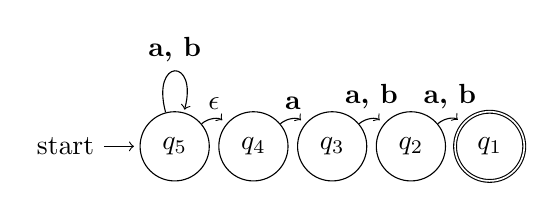
\begin{tikzpicture}
	[shorten >=2pt, on grid,auto] 
   \node[state, initial] (q_1)   {$q_5$}; 
   \node[state] (q_2) [right=of q_1] {$q_4$}; 
   \node[state](q_3) [right=of q_2] {$q_3$};
   \node[state] (q_4) [right=of q_3] {$q_2$};
   \node[state, accepting] (q_5) [right=of q_4] {$q_1$};
    \path[->] 
    (q_1) edge [loop above] node {$\textbf{a, b}$} (q_5)
          edge [bend left=40] node {$\epsilon$} (q_2)
    (q_2) 
          edge [bend left=40] node {$\textbf{a}$} (q_3)
    (q_3) 
          edge [bend left=40] node {$\textbf{a, b}$} (q_4)
    (q_4) 
          edge [bend left=40] node {$\textbf{a, b}$} (q_5);
\end{tikzpicture}

Formally, we can define $N$ as follows:\\

\noindent Let $N = (Q, \Sigma, \delta, q, F)$ recognize $C_k$\\

\indent \textbf{1.} The start state is the start state of $q_{k+1}$\\
\indent \textbf{2.} Following the start state, there are an additional $k$ states\\
\indent \textbf{3.} The accept state is $q_1$\\
\indent \textbf{4.} Define $\delta$ such that \\
\indent\indent $\delta(q_{k+1}, a, b) = q_k$,\\
\indent\indent $\delta(q_{k+1}, \epsilon) = q_k$,\\
\indent\indent $\delta(q_k, a) = q_{k-1}$\\
\indent\indent $\delta(q_{k-n}, a,b) = q_{k-(n+1)}$, where $n \leq (k-1)$\\
 
\paragraph{1.69}  
\mbox{}\\

\noindent \textbf{a.} For the following, the dead state is omitted for clarity, but each state that doesn't have an arrow for 1 or 0 would necessarily go there. The question asks us to show that no DFA will recognize $WW_k$ with fewer than $2^k$ states, we'll start with a diagram. Suppose that $k=1$. We could make the DFA that accepts $WW_k$ as follows, by recognizing that, with a binary alphabet, we can only have the following strings: $\{0,1\}$. The DFA has a minimum of 5 states (with the dead state).\\

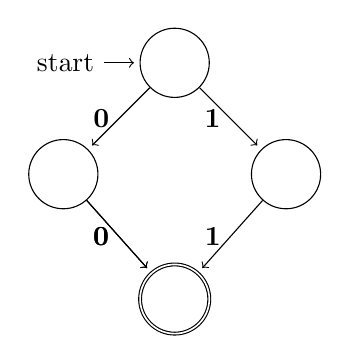
\begin{tikzpicture}
	[shorten >=2pt, on grid,auto, node distance=2cm] 
   \node[state, initial] (q_1)   {}; 
   \node[state] (q_2) [below left=of q_1] {}; 
   \node[state] (q_3) [below right=of q_1] {};
   \node[state, accepting] (q_4) [below=3of q_1] {};
       \path[->] 
    (q_1)
          edge [left=40] node {\textbf{0}} (q_2)
          edge [left=40] node {\textbf{1}} (q_3)
    (q_2) edge [left=40] node {\textbf{0}} (q_4)
    		  edge [left=40] node {\textbf{0}} (q_4)
    (q_3) 
          edge [left=40] node {\textbf{1}} (q_4);
   
\end{tikzpicture}

\mbox{}\\

For $k=2$, we can construct:

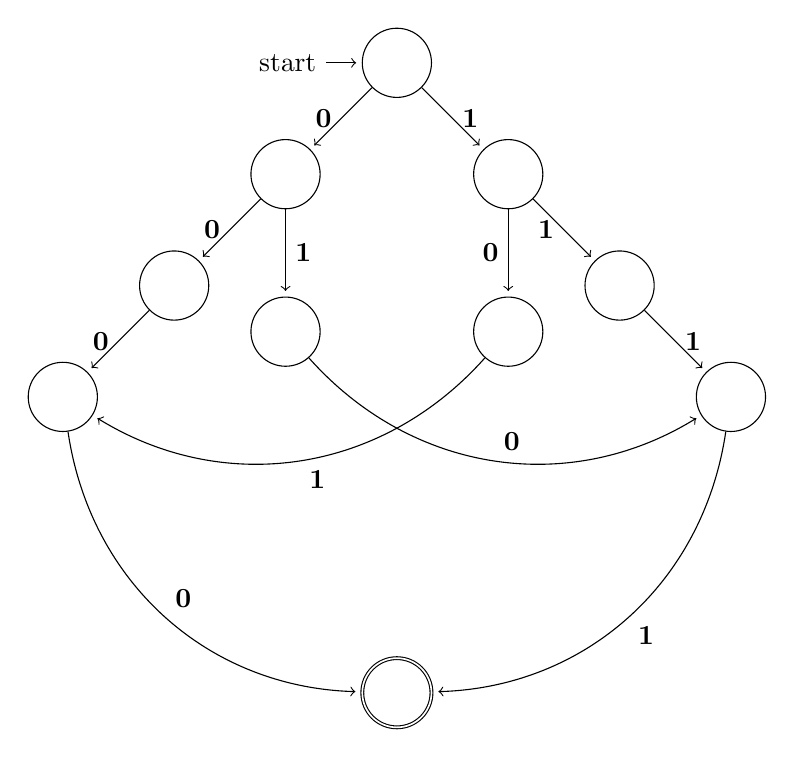
\begin{tikzpicture}
	[shorten >=2pt, on grid,auto, node distance=2cm] 
   \node[state, initial] (q_1)   {}; 
   \node[state] (q_2) [below left=of q_1] {}; 
   \node[state] (q_3) [below right=of q_1] {};
   \node[state, accepting] (q_4) [below=8of q_1] {};
   \node[state] (q_5) [below left=of q_2] {}; 
   \node[state] (q_6) [below right=of q_3] {};
   \node[state] (q_7) [below =2of q_3] {}; 
   \node[state] (q_8) [below =2of q_2] {};
   \node[state] (q_10) [below left =2of q_5] {};
   \node[state] (q_11) [below right =2of q_6] {};
       \path[->] 
    (q_1)
          edge [left=40] node {\textbf{0}} (q_2)
          edge [right=40] node {\textbf{1}} (q_3)
    (q_2) edge [right=40] node {\textbf{1}} (q_8)

    (q_3) edge [left=40] node {\textbf{0}} (q_7)
          edge [left=40] node {\textbf{1}} (q_6)
    (q_2) edge [left=40] node {\textbf{0}} (q_5)
    (q_5) edge [left=40] node {\textbf{0}} (q_10)
    (q_6) edge [right=40] node {\textbf{1}} (q_11)
    (q_7) edge [bend left=40] node {\textbf{1}} (q_10)
    (q_8) edge [bend right=40] node {\textbf{0}} (q_11)
    (q_10) edge [bend right=40] node {\textbf{0}} (q_4)
    (q_11) edge [bend left=40] node {\textbf{1}} (q_4);  
\end{tikzpicture}

Continuing in this fashion, we can continue to increment $k$ by adding more states. These get very complicated very quickly. Here's $k = 3$, (if you can follow the transitions!):\\

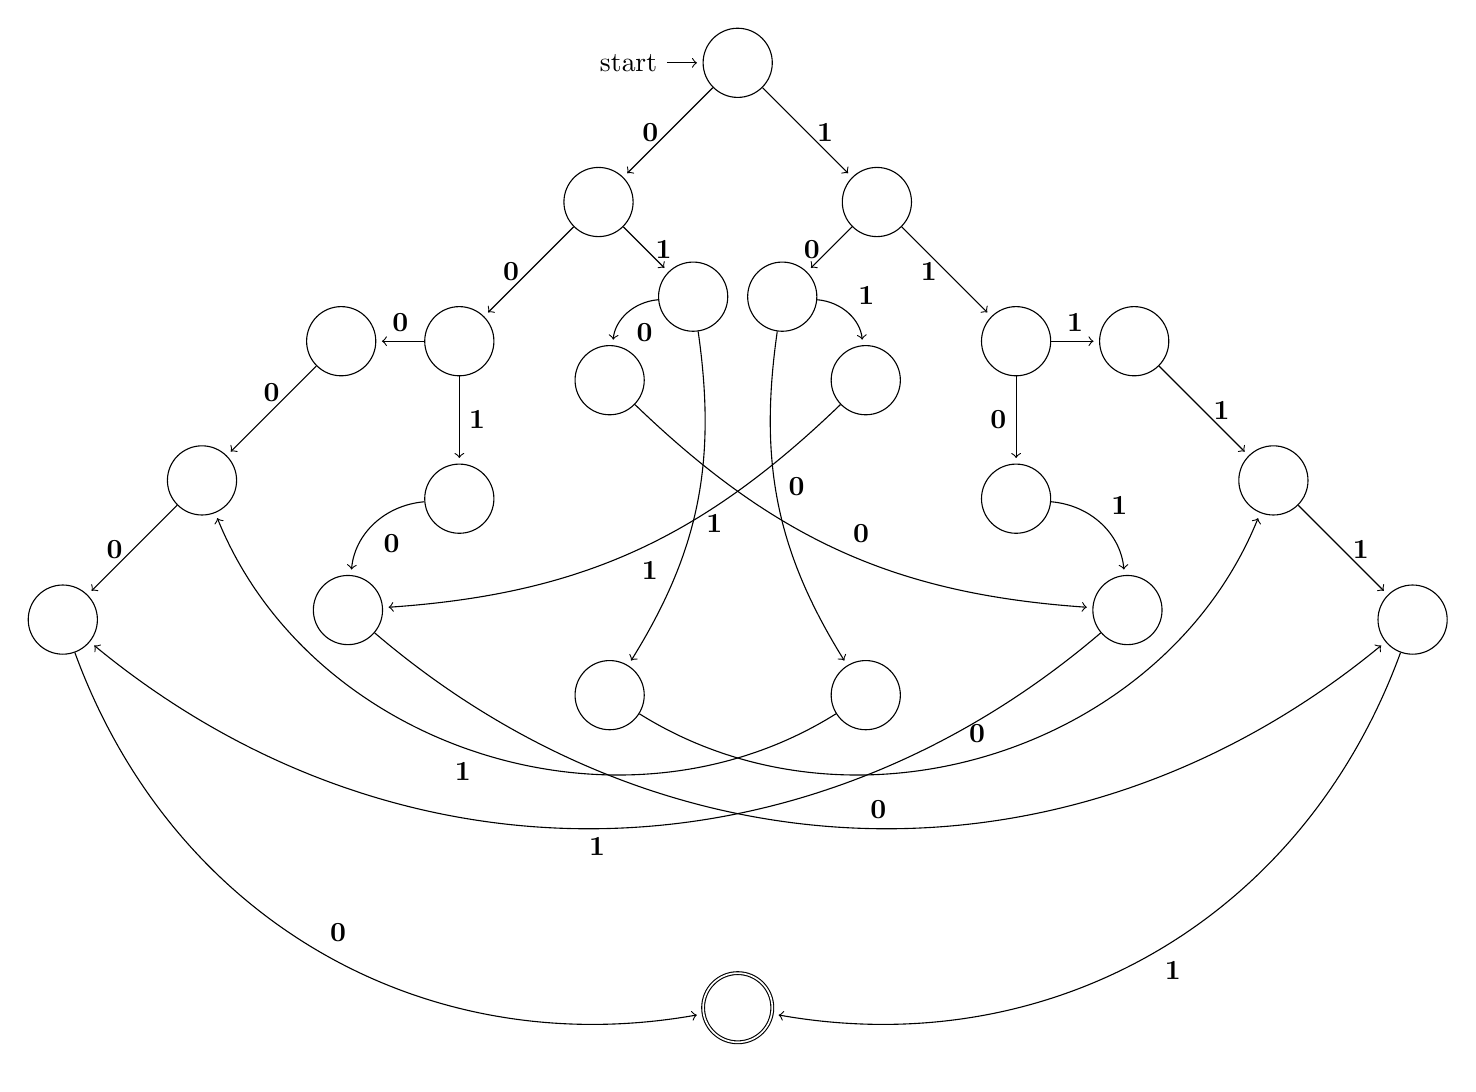
\begin{tikzpicture}
	[shorten >=2pt, on grid,auto, node distance=2cm, minimum size=.5] 
   \node[state, initial] (q_1)   {}; 
   \node[state] (q_2) [below left=2.5of q_1] {}; 
   \node[state] (q_3) [below right=2.5of q_1] {};
   \node[state, accepting] (q_4) [below=12of q_1] {};
   \node[state] (q_5) [below left=2.5of q_2] {}; 
   \node[state] (q_6) [below right=2.5of q_3] {};
   \node[state] (q_7) [below left=1.7of q_3] {}; 
   \node[state] (q_8) [below right=1.7of q_2] {};
   \node[state] (q_10) [left =1.5of q_5] {};
   \node[state] (q_11) [right =1.5of q_6] {};
   \node[state] (q_12) [below left =2.5of q_10] {};
   \node[state] (q_13) [below right =2.5of q_11] {};
   \node[state] (q_14) [below left =2.5of q_12] {};
   \node[state] (q_15) [below right =2.5of q_13] {};
   \node[state] (q_16) [below left =1.5of q_8] {};
   \node[state] (q_17) [below right =1.5of q_7] {};
      \node[state] (q_18) [below =2of q_5] {};
   	  \node[state] (q_19) [below =2of q_6] {};
   	    \node[state] (q_20) [below left =2of q_18] {};
   	  \node[state] (q_21) [below right =2of q_19] {};
   	   \node[state] (q_22) [below =4of q_16] {};
   	  \node[state] (q_23) [below =4of q_17] {};
       \path[->] 
    (q_1)
          edge [left=40] node {\textbf{0}} (q_2)
          edge [right=40] node {\textbf{1}} (q_3)
    (q_2) edge [right=40] node {\textbf{1}} (q_8)
    (q_11) edge [right=40] node {\textbf{1}} (q_13)
   	(q_13) edge [right=40] node {\textbf{1}} (q_15)
   	(q_15) edge [bend left=40] node {\textbf{1}} (q_4)
    (q_3) edge [left=40] node {\textbf{0}} (q_7)
          edge [left=40] node {\textbf{1}} (q_6)
    (q_2) edge [left=40] node {\textbf{0}} (q_5)
    (q_5) edge [above=40] node {\textbf{0}} (q_10)
    edge [right=40] node {\textbf{1}} (q_18)
    (q_14) edge [bend right=40] node {\textbf{0}} (q_4)
        (q_10) edge [above=40] node {\textbf{0}} (q_12)
        (q_12) edge [left=40] node {\textbf{0}} (q_14)
    (q_6) edge [above=40] node {\textbf{1}} (q_11)
    edge [left=40] node {\textbf{0}} (q_19)
    (q_7) edge [bend left=40] node {\textbf{1}} (q_17)
    (q_8) edge [bend right=40] node {\textbf{0}} (q_16)
    (q_18) edge [bend right=40] node {\textbf{0}} (q_20)
    (q_19) edge [bend left=40] node {\textbf{1}} (q_21)
       (q_8) edge [bend left=20] node {\textbf{1}} (q_22)
    (q_7) edge [bend right=20] node {\textbf{0}} (q_23)
       (q_22) edge [bend right=50] node {\textbf{0}} (q_13)
    (q_23) edge [bend left=50] node {\textbf{1}} (q_12)
       (q_20) edge [bend right=40] node {\textbf{0}} (q_15)
    (q_21) edge [bend left=40] node {\textbf{1}} (q_14)
       (q_16) edge [bend right=20] node {\textbf{0}} (q_21)
    (q_17) edge [bend left=20] node {\textbf{1}} (q_20); 
    
\end{tikzpicture}

To see that the DFA will always have more than $2^k$ states, notice that for every $k$, we have to keep track of at least the first $w$ symbols. After the first $w$ symbols, we can reuse some states because they share a substring at the end. But for the first $w$ in $ww$ there are $2^k$ states needed for \textit{each k}, because we add $2^k$ new states for each of the possible binary strings of length $k$. In addition, we must always have an accept state, a start state, and a dead state. Here is the same diagram with the $k^{th}$ level labeling each state that must be added each time $k$ increases:\\

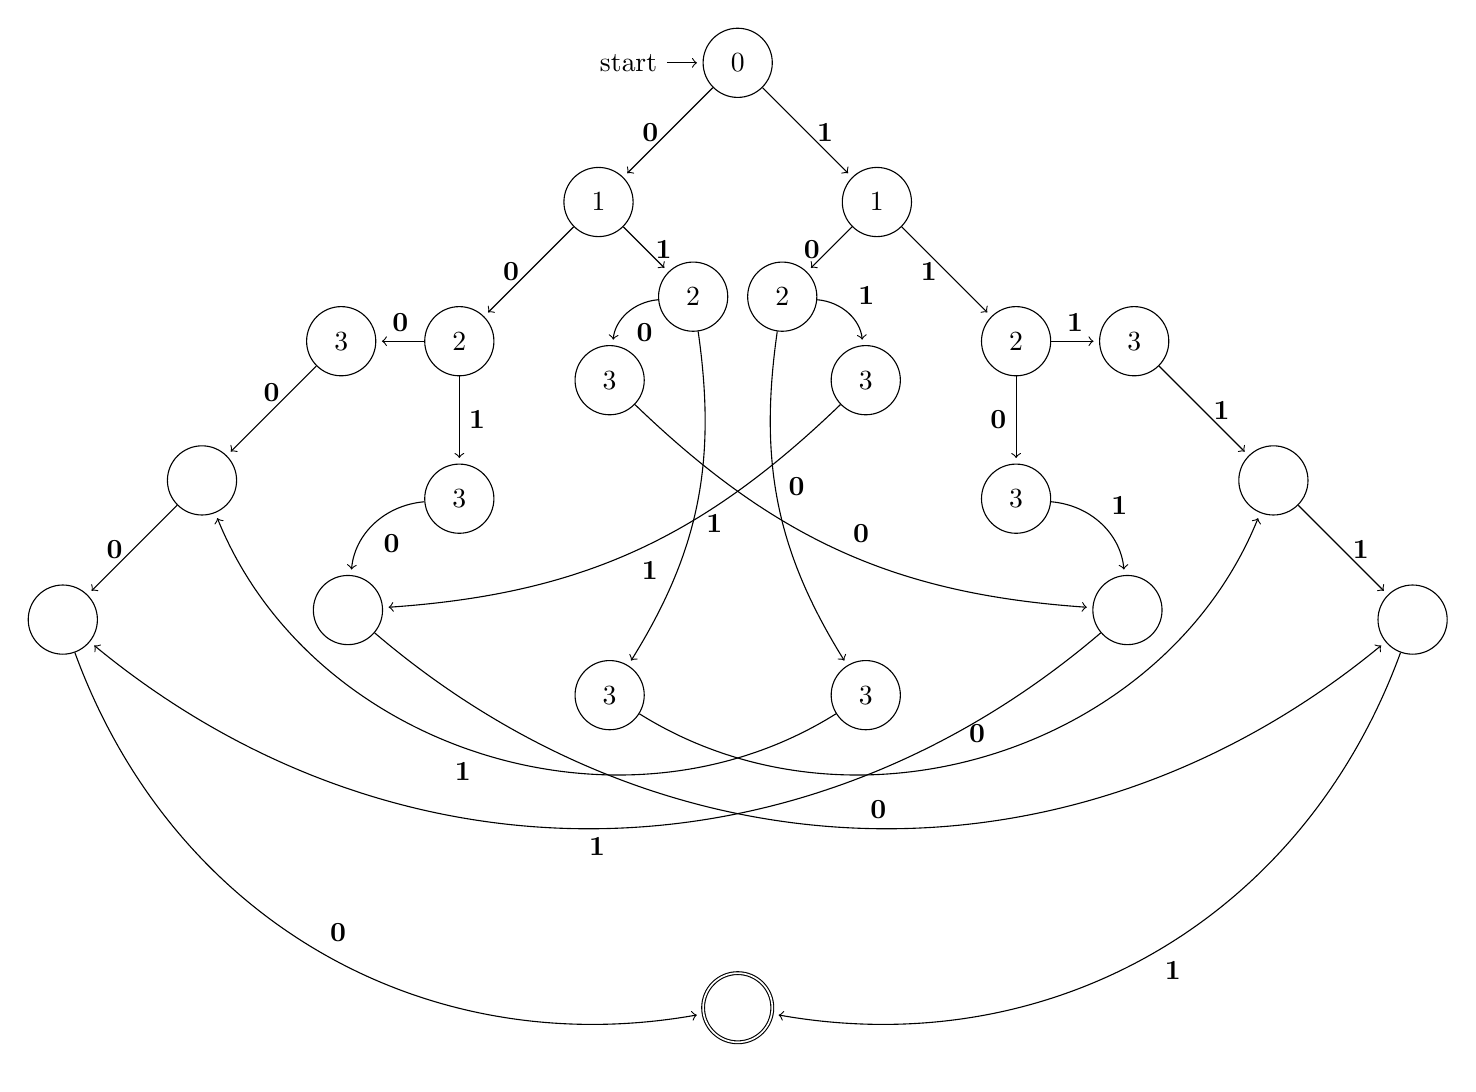
\begin{tikzpicture}
	[shorten >=2pt, on grid,auto, node distance=2cm, minimum size=.5] 
   \node[state, initial] (q_1)   {$0$}; 
   \node[state] (q_2) [below left=2.5of q_1] {$1$}; 
   \node[state] (q_3) [below right=2.5of q_1] {$1$};
   \node[state, accepting] (q_4) [below=12of q_1] {};
   \node[state] (q_5) [below left=2.5of q_2] {$2$}; 
   \node[state] (q_6) [below right=2.5of q_3] {$2$};
   \node[state] (q_7) [below left=1.7of q_3] {$2$}; 
   \node[state] (q_8) [below right=1.7of q_2] {$2$};
   \node[state] (q_10) [left =1.5of q_5] {$3$};
   \node[state] (q_11) [right =1.5of q_6] {$3$};
   \node[state] (q_12) [below left =2.5of q_10] {};
   \node[state] (q_13) [below right =2.5of q_11] {};
   \node[state] (q_14) [below left =2.5of q_12] {};
   \node[state] (q_15) [below right =2.5of q_13] {};
   \node[state] (q_16) [below left =1.5of q_8] {$3$};
   \node[state] (q_17) [below right =1.5of q_7] {$3$};
      \node[state] (q_18) [below =2of q_5] {$3$};
   	  \node[state] (q_19) [below =2of q_6] {$3$};
   	    \node[state] (q_20) [below left =2of q_18] {};
   	  \node[state] (q_21) [below right =2of q_19] {};
   	   \node[state] (q_22) [below =4of q_16] {$3$};
   	  \node[state] (q_23) [below =4of q_17] {$3$};
       \path[->] 
    (q_1)
          edge [left=40] node {\textbf{0}} (q_2)
          edge [right=40] node {\textbf{1}} (q_3)
    (q_2) edge [right=40] node {\textbf{1}} (q_8)
    (q_11) edge [right=40] node {\textbf{1}} (q_13)
   	(q_13) edge [right=40] node {\textbf{1}} (q_15)
   	(q_15) edge [bend left=40] node {\textbf{1}} (q_4)
    (q_3) edge [left=40] node {\textbf{0}} (q_7)
          edge [left=40] node {\textbf{1}} (q_6)
    (q_2) edge [left=40] node {\textbf{0}} (q_5)
    (q_5) edge [above=40] node {\textbf{0}} (q_10)
    edge [right=40] node {\textbf{1}} (q_18)
    (q_14) edge [bend right=40] node {\textbf{0}} (q_4)
        (q_10) edge [above=40] node {\textbf{0}} (q_12)
        (q_12) edge [left=40] node {\textbf{0}} (q_14)
    (q_6) edge [above=40] node {\textbf{1}} (q_11)
    edge [left=40] node {\textbf{0}} (q_19)
    (q_7) edge [bend left=40] node {\textbf{1}} (q_17)
    (q_8) edge [bend right=40] node {\textbf{0}} (q_16)
    (q_18) edge [bend right=40] node {\textbf{0}} (q_20)
    (q_19) edge [bend left=40] node {\textbf{1}} (q_21)
       (q_8) edge [bend left=20] node {\textbf{1}} (q_22)
    (q_7) edge [bend right=20] node {\textbf{0}} (q_23)
       (q_22) edge [bend right=50] node {\textbf{0}} (q_13)
    (q_23) edge [bend left=50] node {\textbf{1}} (q_12)
       (q_20) edge [bend right=40] node {\textbf{0}} (q_15)
    (q_21) edge [bend left=40] node {\textbf{1}} (q_14)
       (q_16) edge [bend right=20] node {\textbf{0}} (q_21)
    (q_17) edge [bend left=20] node {\textbf{1}} (q_20); 
    
\end{tikzpicture}

\noindent \textbf{b.} For the NFA which recognizes the complement of $WW_k$, we have can accept any string that doesn't have length $2k$ (in the upper half of the diagram) and then we can accept any even-length string which doesn't contain a duplicate. Below is the NFA for k=3: 

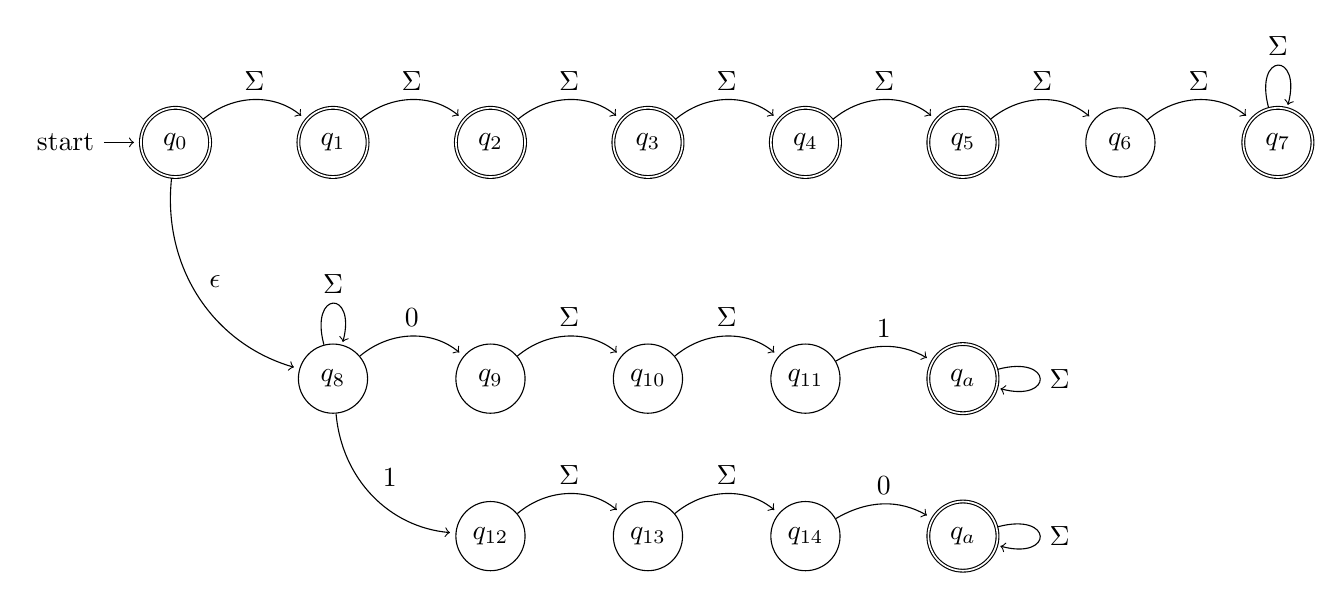
\begin{tikzpicture}
	[shorten >=2pt, on grid,auto,node distance=2cm] 
   \node[initial, state, accepting] (q_0) {$q_{0}$}; 
    \node[state, accepting] (q_1) [right=of q_0]{$q_{1}$}; 
   \node[state, accepting] (q_2) [right=of q_1] {$q_{2}$}; 
   \node[state, accepting] (q_3) [right=of q_2] {$q_{3}$};
   \node[state, accepting] (q_4) [right=of q_3] {$q_{4}$};
   \node[state, accepting] (q_5) [right=of q_4] {$q_{5}$}; 
   \node[state] (q_6) [right=of q_5] {$q_{6}$};
   \node[state, accepting] (q_7) [right=of q_6] {$q_{7}$};
   \node[state] (q_8) [below=3of q_1] {$q_{8}$}; 
   \node[state] (q_9) [right=of q_8] {$q_{9}$};
   \node[state] (q_10) [right=of q_9] {$q_{10}$};   			      \node[state] (q_11) [right=of q_10] {$q_{11}$}; 
   \node[state] (q_12) [below=of q_9] {$q_{12}$};
   \node[state] (q_13) [right=of q_12] {$q_{13}$};
   \node[state] (q_14) [right=of q_13] {$q_{14}$};
   \node[state, accepting] (q_15) [right=of q_11] {$q_{a}$};
   \node[state, accepting] (q_16) [right=of q_14] {$q_{a}$};
 
    \path[->] 
 
   (q_0) 
          edge [bend left=40] node {$\Sigma$} (q_1)
            edge [bend right=40] node {$\epsilon$} (q_8)
          
    (q_1) 
  
          edge [bend left=40] node {$\Sigma$} (q_2)
       
    (q_2) 
          edge [bend left=40] node {$\Sigma$}(q_3)
          
    (q_3) 
          edge [bend left=40] node {$\Sigma$} (q_4)
       
    (q_4) 
          edge [bend left=40] node {$\Sigma$} (q_5)
     
    (q_5) edge [bend left=40] node {$\Sigma$} (q_6)
   
    (q_6) edge [bend left=40] node {$\Sigma$} (q_7)
    (q_7) 
     	  edge [loop above] node {$\Sigma$} (q_7)
    (q_8) 
          edge [bend left=40] node {$0$} (q_9)
          edge [bend right=40] node {$1$} (q_12)
          edge [loop above] node {$\Sigma$} (q_8)
    (q_9) 
          edge [bend left=40] node {$\Sigma$} (q_10)
              (q_12) 
          edge [bend left=40] node {$\Sigma$} (q_13)
              (q_10) 
          edge [bend left=40] node {$\Sigma$} (q_11)
          (q_11)
          edge [bend left] node {$1$} (q_15)
              (q_13) 
          edge [bend left=40] node {$\Sigma$} (q_14)
          	(q_14)
          edge [bend left] node {$0$} (q_16)
          (q_15)
          edge [loop right] node {$\Sigma$} (q_15)
          (q_16)
          edge [loop right] node {$\Sigma$} (q_16);

\end{tikzpicture}


\end{document}  

